%%%%%%%%%%%%%%%%%%%%%%%%%%%%%%%%%%%%%%%%%%%%%%%%%%%%%%%%%%%%%%%%%%%%%%%%%%%%%%%%
\chapter{Εισαγωγή}

Πολλοί παράγοντες συμβάλουν στην συντεταγμένη κίνηση του σώματος και η γοητεία των επιστημόνων έχει οδηγήσει σε αμέτρητα πειράματα και μελέτες ώστε να μπορούν να την εξηγήσουν. Ως αποτέλεσμα υπάρχει πληθώρα υλικό και αποτελέσματα από μελέτες των χαρακτηριστικών των μυών του σώματος, την γεωμετρική τους συσχέτιση με τα οστά και το αποτέλεσμα της κίνησης των αρθρώσεων. Κατά καιρούς έχουν γίνει κλινικές μελέτες σε ασθένειες όπως είναι η εγκεφαλική παράλυση, το εγκεφαλικό επεισόδιο, η οστεοαρθρίτιδα, η Νόσο του Πάρκινσον ώστε να μελετηθούν οι νευρικές διεγέρσεις που οδηγούν την κίνηση του σώματος τόσο πριν την θεραπεία αλλά και μετά, με σκοπό να εξαχθούν συμπεράσματα για την αντιμετώπιση τους. Δυστυχώς η σύνθεση των δεδομένων από τις κλινικές μελέτες για την κατανόηση της δυσλειτουργίας που οφείλεται στην ασθένεια και την δημιουργία μια επιστημονικής βάσης για την αντιμετώπιση της ανώμαλης κίνησης παραμένει μια σημαντική πρόκληση.

Η χρήση πειραμάτων για την κατανόηση της δυναμικής της κίνησης έχει κάποια μειονεκτήματα. Για παράδειγμα η εκτίμηση των δυνάμεων που παράγονται από τους μύες είναι ακατόρθωτο να μετρηθούν πειραματικά. Επίσης υπάρχει δυσκολία κατανόησης των φαινομένων δράσης-αντίδρασης σε τόσο πολύπλοκα συστήματα μόνο από πειράματα. Ο προσδιορισμός της συνεισφοράς κάθε μυ στην κίνηση δεν είναι προφανές γιατί πολλές φορές η δράση του δεν συνεπάγεται μόνο την επιτάχυνση της άρθρωσης στην οποία δρα \cite{zajac-gordon89} αλλά και σε άλλες αρθρώσεις.

Απαραίτητη προϋπόθεση για την μελέτη πολύπλοκων διατάξεων είναι η ανάπτυξη θεωρητικών μοντέλων που μπορούν να προσεγγίσουν τις ανθρώπινες δραστηριότητες και σε συνδυασμό με τις πειραματικές ενδείξεις να γίνει συστηματική μελέτη. Το σύστημα θα πρέπει να είναι σε θέση να φανερώσει τις εξαρτήσεις μεταξύ του νευρικού, του μυϊκού, του σκελετικού συστήματος και της κίνησης του σώματος. Είναι φανερό ότι τα αποτελέσματα αυτού του είδους αναλύσεων παρέχουν μεγαλύτερη πληροφορία και δίνουν την δυνατότητα στους ερευνητές να εξάγουν κατάλληλη θεραπεία για την ασθένεια.

Τα τελευταία χρόνια και ιδιαίτερα με την ανάπτυξη των υπολογιστών ήμαστε σε θέση να κάνουμε πολύπλοκες προσομοιώσεις σε μικρότερο χρονικό διάστημα (της τάξεων μερικών ωρών) που πριν μια δεκαετία θα χρειαζόταν και μέρες. Ο παράγοντας που βελτιώσε την δραματική μείωση του χρόνου δεν οφείλεται μόνο στην ανάπτυξη των υπολογιστών αλλά και στην εφεύρεση νέων μεθόδων. Η δυναμική προσομοίωση και την ανάπτυξη μυοσκελετικών αλλά και νευρομυοσκελετικά μοντέλων είναι σε θέση να δώσουν λύση σε πολλά προβλήματα που απασχολούν την ιατρική και είναι ευρέως αποδεχτά και έχουν μελετηθεί σε βάθος \cite{thelen-chumanov06, piazza06, pandy01, zajac02}.

Παρόλα αυτά υπάρχουν πολλά προβλήματα και φαινόμενα που δεν έχουν μοντελοποιηθεί ώστε να δώσουν πρόγνωση. Τα μοντέλα που έχουν δημιουργηθεί δεν είναι τόσο ακριβή και υπάρχει περιθώριο βελτιώσεων. Επίσης σε κάποιες αναλύσεις εκτελούνται ακόμα με απαγορευτικούς χρόνους κάνοντας τα ακατάλληλα πολλές φορές. Μεγάλη πρόοδος έχει γίνει στην ανάπτυξη αξιόπιστων μοντέλων για τον μυ, αλλά η μεγάλη διαφοροποίηση που υπάρχει στο ανθρώπινο σώμα καθιστά δύσκολη την χρήση ενός γενικού μοντέλου. Από την άλλη υπάρχει μεγάλο χάσμα στην διασύνδεση του νευρικού συστήματος με το κινητήριο σύστημα και τα μοντέλα που υπάρχουν είναι απλοποιημένα και δεν αναπαριστούν πλήρες τις λειτουργίες του. Συμπερασματικά πρέπει να γίνει πολύ δουλεία τόσο από την μεριά των επιστημόνων που μελετούν την ανθρώπινη φυσιολογία αλλά και των μηχανικών που μοντελοποιούν τα συστήματα ώστε να τα χρησιμοποιήσουν στις προσομοιώσεις.

Είναι αναγκαία η δημιουργία ενιαίων εργαλείων και μοντέλων που θα χρησιμοποιούνται από την επιστημονική κοινότητα στις μελέτες τους. Υπάρχουν πολλά εργαστήρια που έχουν αναπτύξει ενδιαφέρουσες τεχνικές, ωστόσο τα αποτελέσματα τους δεν είναι διαθέσιμα για να χρησιμοποιηθεί από άλλους. Υπάρχουν αρκετά εμπορικά εργαλεία (\eng{Anybody, Adams, Visuals 3D}) που είναι κλειστού κώδικα και δεν δίνουν την δυνατότητα επέκτασης και ευελιξίας. Η ανάγκη αυτή έχει οδηγήσει στην ανάπτυξη του ανοιχτού συστήματος \eng{OpenSim} που υποστηρίζεται από μια μεγάλη κοινότητα με πολλά μοντέλα και αναλυτικές μεθόδους, έχοντας βοηθήσει σημαντικά τους ερευνητές τα τελευταία χρόνια. Δίνοντας την δυνατότητα στους επιστήμονες να μοιράζονται κοινές μεθόδους ανάλυσης, μοντέλα και αποτελέσματα, βοηθάει στην βελτίωση, στην αναπαραγωγή και επιβεβαίωση των αποτελεσμάτων που έχουν εξαχθεί από τρίτους.

%%%%%%%%%%%%%%%%%%%%%%%%%%%%%%%%%%%%%%%%%%%%%%%%%%%%%%%%%%%%%%%%%%%%%%%%%%%%%%%%
\section*{Παραδείγματα}

Ως κλασικό παράδειγμα θα αποδείξουμε ότι τα μυοσκελετικά μοντέλων μπορούν να χρησιμοποιηθούν για να εκτιμηθεί η πορεία θεραπείας ορθοπεδικών εγχειρήσεων. Η βάδιση με λυγισμένα τα γόνατα (\eng{crouch gait}) είναι μια από τις πιο κοινές ανωμαλίες σε άτομα με εγκεφαλική παράλυση. Χαρακτηριστικό αυτής της βάδισης είναι το περπάτημα με λυγισμένα γόνατα και η ανικανότητα να παραχθεί αρκετή δύναμη από τους μύες στο γόνατο ώστε να σηκωθεί η λεκάνη (μια κίνηση που απαιτεί πολύ δύναμη και κόπωση από τους μύες).  Μια αιτία είναι το μικρό μήκος του Ημιτενοντώδη μυ και μερικές φορές η θεραπεία είναι η επιμήκυνση του μυ. Ωστόσο, μπορούν να υπάρχουν και άλλες αιτίες της υπερβολικής κάμψης του γόνατος (π.χ. αδύναμοι καμπτήρες της ποδοκνημικής άρθρωσης), και η επιμήκυνση του Ημιτενοντώδη μπορεί να θέσει σε κίνδυνο την αντοχή των μυών στον αστράγαλο \cite{arnolda06}.

\begin{figure}[H]
    \centering
    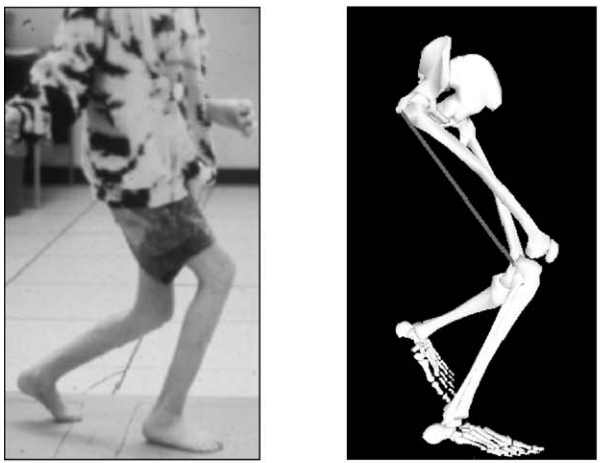
\includegraphics[width=0.8\textwidth]{introduction/fig/crouch-gait.png}
    \caption{Πρόβλημα περπατήματος με λυγισμένα γόνατα\cite{arnolda06}}
    \label{fig:crouch-gait}
\end{figure}

Για αυτό το λόγο μπορούν να γίνουν καταγραφές της βάδισης του ασθενή σε ειδικά εργαστήρια και με κατάλληλο μοντέλο των κάτω άκρων και να μελετηθεί για τον συγκεκριμένο ασθενή αν πρέπει να γίνει η επιμήκυνση του Ημιτενοντώδη. Στα μοντέλα είναι δυνατή η παραμετροποίηση των μυών για το συγκεκριμένο ασθενή ώστε να μελετηθεί με ορθή δυναμική το αποτέλεσμα της εγχείρισης εικονικά. Τέτοιου είδους αναλύσεις θα ήταν ένα χρήσιμο εργαλείο για τους ιατρούς ώστε να τους δώσουν μια εποπτική κατάσταση του ασθενή, να βελτιώσουν την επιτυχία της εγχείρισης αλλά και την δημιουργία μιας θεραπευτικής αγωγής.

Ως δεύτερο παράδειγμα \cite{fregly07} είναι η μελέτη τόπου βαδίσματος ώστε να μειωθεί η καταπόνηση του γονάτου. Σε αυτή την μελέτη οι ασθενείς με προβλήματα οστεοαρθρίτιδα καταπονούν το γόνατο κατά την βάδιση, οπότε οι συγγραφείς προτείνουν μια πολύ απλή παραλλαγή της βάδισης ώστε να μειωθεί η δύναμη που ασκείται στο γόνατο, στρέφοντας ελαφρά το πόδι προστάξω. Κατά το πείραμα οι ασθενείς καταγράφονται από συστήματα παρακολούθησης της κίνησης και επίσης καταγράφεται η αντίδραση εδάφους. Εφαρμόζεται αντίστροφη κινηματική και αντίστροφη δυναμική και σε πραγματικό χρόνο υπάρχει μέτρηση της δύναμης που ασκείται στο γόνατο αλλά και του προσανατολισμού του ποδιού. Στα πλαίσια του πειράματος έχει αναπτυχθεί μια συσκευή που σηματοδοτεί τον ασθενή όταν δεν ακολουθεί τους κανόνες της βάδισης για την μείωση της καταπόντισης. Ως αποτέλεσμα μετά από τέσσερα σεμινάρια οι ασθενείς είχαν συνηθίσει στο νέο τρόπο βάδισης ώστε να μην καταπονούν το γόνατο.

\begin{figure}[H]
    \centering
    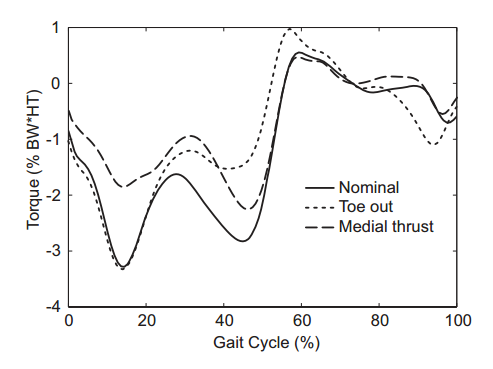
\includegraphics[width=0.8\textwidth]{introduction/fig/knee-load.png}
    \caption{Αποτελέσματα της ροπής της προσαγωγή στο γόνατο\cite{fregly07}}
    \label{fig:knee-load}
\end{figure}

Σαν τρίτο παράδειγμα, θα ήταν ενδιαφέρον να μπορούσαμε να μελετήσουμε την συμπεριφορά των φαρμάκων στις ασθένειες και δραστηριότητες των ανθρώπων. Ως βασικό προαπαιτούμενο απαιτείται η κατανόηση και η μοντελοποίηση της δράσης του φαρμάκου ώστε να μπορεί να προσομοιωθεί. Επίσης απαιτείται η μοντελοποίηση της ασθένειας και το πως αυτή συνδέεται με τις δραστηριότητες του ανθρώπου. Έχουν γίνει μελέτες μοντελοποίησης φαρμάκων όπως είναι η δοπαμίνη για την θεραπεία της Νόσος του Πάρκινσον \cite{haeri05}. Ωστόσο, υπάρχουν δυσκολίες όπως είναι η μοντελοποίηση του βασικά γάγγλια (\eng{basal ganglia}). Παρόλο αυτά μπορούν να εξαχθούν ενδιαφέροντα αποτελέσματα και να εξηγηθούν πράγματα που ίσως δώσουν λύση στην εύρεση μεθόδων θεραπείας δύσκολων ασθενειών.

Συμπερασματικά, οι προσομοιώσεις μπορούν να βοηθήσουν την επιστήμη της ιατρικής και όχι μόνο στο να μελετά την συμπεριφορά μια ασθένειας αλλά και να εξάγει συμπεράσματα θεραπείας και στρατηγικές αγωγής. Οι μέθοδοι προσομοιώσεων χρησιμοποιούνται σε άλλες βιομηχανίες, όπως είναι η βιομηχανία των αυτοκινήτων για την σχεδίαση κινητήρων και έχει μειώσει δραματικά το κόστος κατασκευής τους. Ως εκ τούτου θα πρέπει να χρησιμοποιούνται και στην ιατρική, στην παραγωγή νέων φαρμάκων, την δημιουργία νέων ορθοπεδικών μηχανισμών όπως είναι οι υποστηρικτές σκελετικού συστήματος \cite{stopforth12} και σε πολλούς άλλους κλάδους.
